\documentclass[conference]{IEEEtran}
\IEEEoverridecommandlockouts

\usepackage{cite}
\usepackage{amsmath,amssymb}
\usepackage{graphicx}
\usepackage{booktabs}
\usepackage{url}
\usepackage{balance}

\graphicspath{{./figures/}{./}}

\begin{document}

\title{AvenaRS: A Deployed Edge Camera and Sensor System for Lane-Level Pavement Load Monitoring}

\author{\IEEEauthorblockN{Andrew D. Balmos, Anuska Das, Anugunj Naman, Spencer Beane, Yaguang Zhang, James V. Krogmeier}
\IEEEauthorblockA{Purdue University, West Lafayette, Indiana, USA}
\thanks{This work was supported by JTRP SPR-4918: ``Enhancing Pavement Instrumentation and Monitoring: A Novel Edge First, Network-Level Solution for Pavement and Roadside Sensors with Live Data Visualization.''}}

\maketitle

\begin{abstract}
Pavement sections instrumented with embedded pressure, strain, and environmental sensors can provide high-value structural insight, but many deployments still rely on sparse collection campaigns and lack synchronized vehicle context. This limits event-level interpretation and weakens decision support for proactive maintenance. We present Avena Road Side (AvenaRS), an edge-native multimodal system that continuously acquires embedded sensor signals and binds them to lane-level vehicle events derived from roadside cameras. The implemented stack combines Rust-based acquisition services, Python camera analytics, NATS/JetStream messaging, calibration-aware Parquet archival, and a web dashboard for remote configuration, trigger visualization, and historical export. This work is presented as a deployed systems contribution: we document the end-to-end architecture, network-wide multi-site operation, solar-aware field design, and deployment evidence from I-65 and APT pilots with emphasis on continuity, recoverability, and operational usability. The central innovation is a unified sensing-to-action path in real roadway environments, enabling lane-level pavement event monitoring without site-specific custom integration.
\end{abstract}

\begin{IEEEkeywords}
pavement monitoring, edge computing, roadside sensing, vehicle tracking, NATS, LabJack, multimodal telemetry
\end{IEEEkeywords}

\section{Introduction}
Embedded pavement instrumentation is widely recognized as a path to higher-fidelity structural monitoring than periodic manual inspection \cite{Barriera2020SituPavementMonitoring, Xin2025}. However, many practical deployments still operate as disconnected subsystems: sensor data are collected in campaigns, vehicle context is inferred indirectly, and cross-modal alignment is left to offline analysis. This creates two major constraints for transportation agencies. First, sparse collection windows reduce temporal coverage of deterioration processes. Second, lack of synchronized vehicle metadata (lane, speed, axle/wheel timing proxies) limits comparability of loading events and weakens condition inference for prioritization workflows \cite{Jha2023DataDrivenWeb}.

Prior work has established the value of in-situ sensing, IoT monitoring, and continuous structural data collection \cite{Xue2014PavementHealthMonitoring, Alavi2016Continuoushealthmonitoring, Ceylan2016FieldDemo, Micko2023, Liu2024SensorBasedStructural, Ye2024}. A remaining systems gap is an operationally deployable architecture that jointly handles sensor telemetry, camera analytics, remote control, calibration lineage, and export at roadway scale.

AvenaRS addresses that gap by integrating sensor and camera pipelines into a single edge-first cyber-physical stack built on Avena principles \cite{avena2022, castiblanco2024avena, castiblanco2024oatsmobile, gowda2025enhancing}. The contribution is not an isolated detector improvement; it is an implemented and remotely operable end-to-end system that preserves event semantics from roadside acquisition through archival and user-facing data products.

This paper makes three contributions:
\begin{itemize}
\item an implementation-grounded architecture for fused sensor-camera roadside monitoring with dynamic reconfiguration;
\item a deployment evaluation framework centered on operational continuity, observability, and recoverability;
\item network-wide and solar-aware design choices demonstrated through I-65 and APT field deployments.
\end{itemize}

\section{System Design and Implementation}
\subsection{Deployed edge topology and software roles}
AvenaRS is deployed as a roadside edge node connected to embedded analog sensors, IP cameras, local storage, and upstream connectivity. Current hardware centers on a LabJack T7 OEM module (a commercial multi-channel analog data-acquisition unit) \cite{labjack_t7_datasheet} and an x86 embedded host (LattePanda Sigma) \cite{lattepanda:sigma:datasheet}. The software stack consists of five cooperating components: \texttt{streamer}, \texttt{archiver}, \texttt{exporter}, camera analytics services, and a web dashboard client.

\begin{figure}[t]
\centering
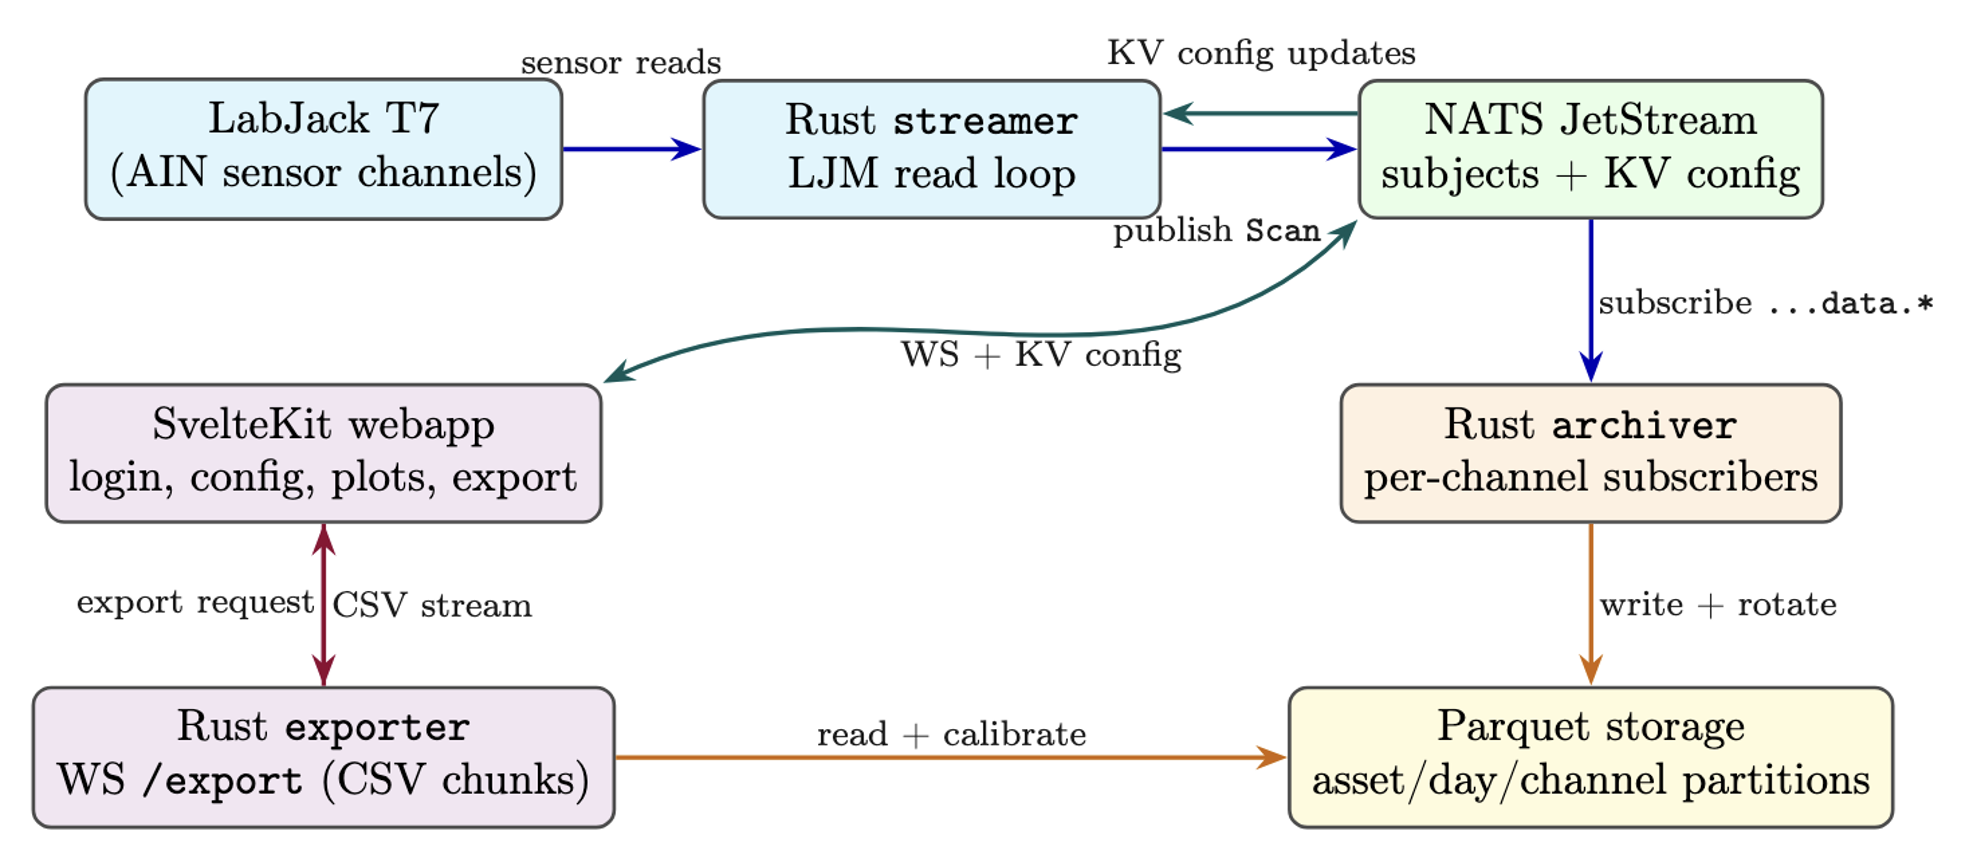
\includegraphics[width=0.98\linewidth]{overview.png}
\caption{AvenaRS application overview from deployed software components: LabJack acquisition, streaming, JetStream transport, archival, export, and SvelteKit operations interface.}
\label{fig:system_overview}
\end{figure}

Sensor and camera services publish events to the same message fabric so downstream consumers can subscribe by semantic subject instead of process-local APIs. This reduces coupling and allows runtime updates without redeploying the full node.

\subsection{Network-wide multi-site architecture}
The deployment model is designed for statewide scale rather than a single roadside cabinet. Each AvenaRS site operates as an autonomous edge node for sensing and local processing, while simultaneously participating in a network-wide system for remote monitoring, configuration, and data access. This architecture allows operations teams to manage many instrumented sites through a central service layer without removing local autonomy when connectivity is limited.

\begin{figure}[t]
\centering
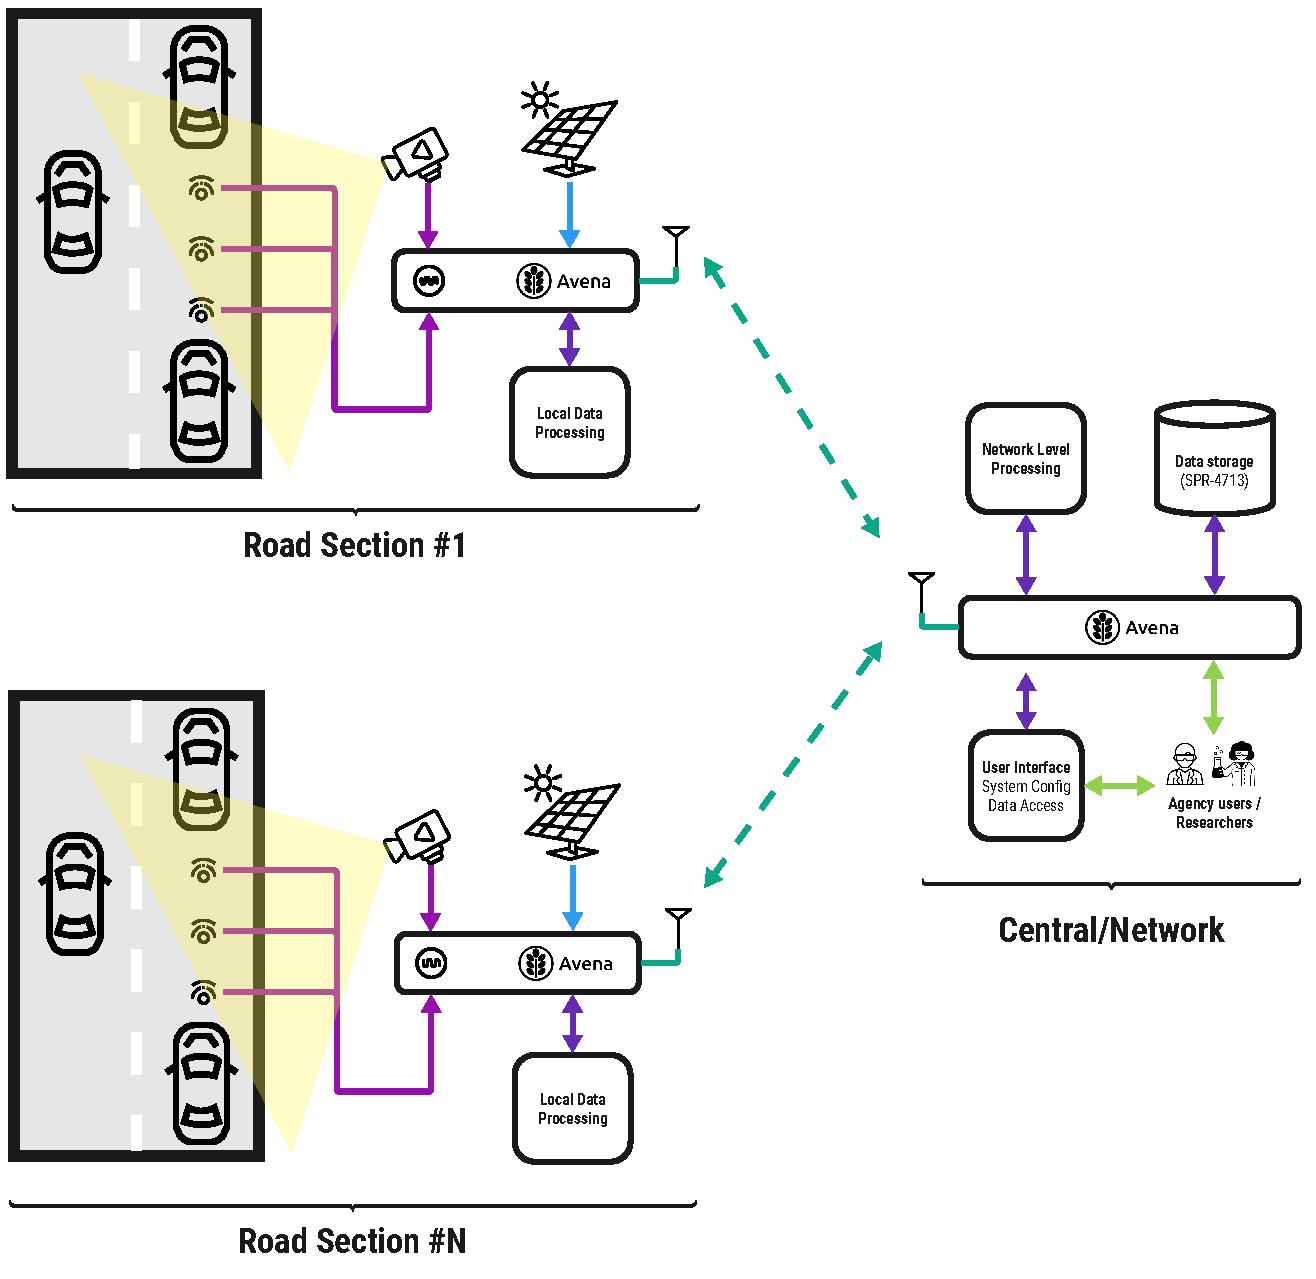
\includegraphics[width=0.95\linewidth]{AvenaRS.pdf}
\caption{Individual AvenaRS devices participating in a network-wide system with central monitoring and control.}
\label{fig:network_arch}
\end{figure}

This structure supports two complementary functions: local continuity for resilient roadside operation and centralized coordination for statewide analytics and maintenance planning.

\subsection{Sensor acquisition and event transport}
The \texttt{streamer}, implemented in Rust (a systems programming language), loads channel configuration from JetStream KV, opens the LabJack over configurable transport order (Ethernet/USB), and publishes per-channel FlatBuffer scan messages \cite{google_flatbuffers}. Subjects are content-addressed by asset and channel:
\begin{equation}
S_{a,c} = p.\texttt{asset}_a.\texttt{data}.\texttt{ch}_c,
\end{equation}
where $p$ is a subject prefix, $a$ is zero-padded asset number, and $c$ is zero-padded channel number. This pattern supports selective subscriptions and wildcard fan-out under NATS routing \cite{nats_io}.

The \texttt{archiver} consumes channel subjects and writes partitioned Parquet files (columnar analytics format) using
\path{parquet/assetNNN/YYYY-MM-DD/chCC/part-XXXX.parquet}. 
Each file stores calibration metadata (identity, linear, or polynomial) so historical exports remain reproducible even when calibration presets change later.

\subsection{Camera analytics and lane-level event extraction}
The camera pipeline supports two complementary modes. The primary mode uses YOLO-based detection/tracking for vehicle IDs, lane polygons, and crossing events. A fallback mode uses dense optical flow plus SORT tracking for motion-centric operation when detector assumptions are violated \cite{Farnebaeck2003, bewley2016}. For each track, a 1D constant-velocity Kalman filter estimates front-edge kinematics and crossing interpolation:
\begin{equation}
\hat{t}_{\mathrm{cross}} = t_{k-1} + \frac{x_{\mathrm{cross}}-x_{k-1}}{x_k-x_{k-1}}(t_k-t_{k-1}).
\end{equation}

Wheel-event refinement is then computed around the crossing window by clustering front-to-wheel longitudinal offsets, yielding wheel crossing estimates:
\begin{equation}
\hat{t}_{\mathrm{wheel},i} = \hat{t}_{\mathrm{front}} + \frac{\Delta x_i}{\hat{v}_x}.
\end{equation}

These events provide a practical bridge from image-space motion to load-aligned sensor interpretation.

\subsection{Operations interface and remote control surface}
The operations dashboard is built with SvelteKit (a JavaScript/TypeScript web application framework) and provides credentialed NATS connection, KV-backed LabJack configuration CRUD, calibration preset management, real-time waveform display, trigger modes, and historical export via WebSocket CSV streaming. This interface is essential for deployment because validation and maintenance are executed by multidisciplinary teams (research staff, field technicians, and agency operators), not only model developers.

\begin{figure}[t]
\centering
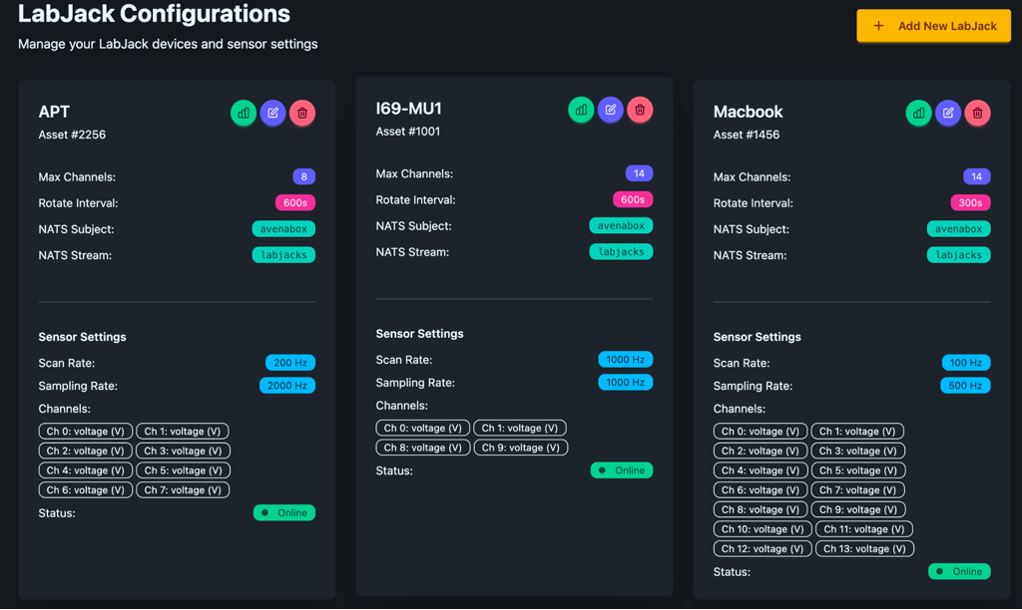
\includegraphics[width=0.98\linewidth]{ss_1.png}
\caption{Web dashboard configuration surface used in deployment: asset status, channel selection, sampling rates, and stream configuration management.}
\label{fig:webapp_config}
\end{figure}

\begin{figure}[t]
\centering
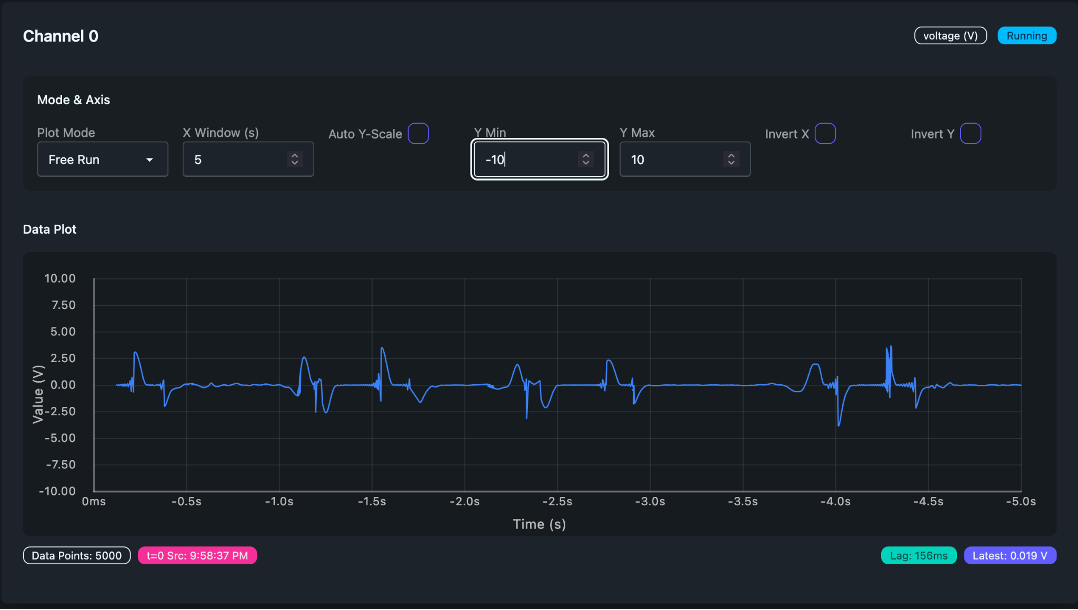
\includegraphics[width=0.98\linewidth]{ss_2.png}
\caption{Web dashboard live plot surface used for trigger validation, channel health checks, and short-window diagnostics during field operation.}
\label{fig:webapp_plot}
\end{figure}

\section{Deployment Evaluation Methodology}
\subsection{Evaluation objective and scope}
This paper evaluates AvenaRS as an infrastructure deployment system rather than a model-benchmark study. The objective is to determine whether the deployed stack can sustain lane-level sensing workflows under practical roadside constraints while remaining observable, diagnosable, and operable by a multidisciplinary operations team.

We structure evaluation around five deployment evidence dimensions:
\begin{itemize}
\item \textbf{Acquisition continuity}: whether camera and sensor ingestion remain active through routine runtime disturbances.
\item \textbf{End-to-end observability}: whether events remain traceable from source acquisition to archival and export.
\item \textbf{Remote operability}: whether operators can safely modify configuration and confirm behavior through the dashboard.
\item \textbf{Failure recoverability}: whether service interruptions are detected, isolated, and recovered without data-pipeline collapse.
\item \textbf{Cross-site transferability}: whether one software stack can be reused across open-road and controlled environments.
\end{itemize}

This scope matches the current project stage, where deployment reliability and system integration are primary prerequisites for long-duration field studies.

\subsection{Evidence sources and instrumentation surfaces}
Evidence is collected from native process telemetry rather than additional post hoc instrumentation. The Rust \texttt{streamer} and \texttt{archiver} provide channel-level acquisition, write, and partition logs; camera analytics services emit lane/crossing events with track identifiers; JetStream subjects record publish and subscribe activity; and the dashboard plus exporter provide control-action and export traces.

To preserve lineage across these surfaces, each event record is tied to a compact provenance tuple:
\begin{equation}
\ell(e)=\{a,c,s,t,r\},
\end{equation}
where $a$ is asset identifier, $c$ is channel or camera stream identifier, $s$ is message subject, $t$ is event timestamp, and $r$ is configuration revision. This representation makes field debugging and replay analysis practical even when multiple services are restarted during operation.

\subsection{I-65 and APT field protocol}
The protocol uses two complementary contexts: (i) I-65 roadside pilot operation and (ii) controlled APT campaigns. I-65 captures realistic disturbances such as changing traffic mix, lighting transitions, camera-stream instability, and intermittent network quality. APT provides repeatable geometry and controlled vehicle movement, which is useful for regression checks after software or configuration updates.

Each run follows a fixed sequence: pre-run configuration push, live signal verification in the dashboard, continuous acquisition with passive monitoring, event and storage health checks, and post-run export verification. This sequence is aligned with routine deployment practice so that evaluation reflects operational maintenance conditions rather than isolated laboratory procedures.

\section{Field Deployment Evidence (I-65/APT)}
Table~\ref{tab:deployment_evidence} summarizes deployment evidence across the two pilot environments.

\begin{table}[t]
\caption{Deployment evidence summary from I-65 roadside and APT controlled pilots.}
\label{tab:deployment_evidence}
\centering
\footnotesize
\begin{tabular}{@{}p{0.18\linewidth}p{0.34\linewidth}p{0.34\linewidth}@{}}
\toprule
Dimension & I-65 roadside pilot & APT controlled pilot \\
\midrule
Acquisition continuity & Continuous ingest through transient camera and network jitter; services maintained stream continuity after reconnect. & Repeatable ingest across controlled runs with consistent startup and shutdown behavior. \\
Remote operability & Live dashboard updates for channels, rates, and stream parameters during active operation with immediate status feedback. & Fast parameter sweeps and configuration turnover for scenario-based experiments. \\
Event-to-storage traceability & Camera and sensor events retained consistent subject lineage and partitioned archival paths for replay. & Deterministic replay windows confirmed that software revisions preserved event semantics. \\
Failure recoverability & Watchdog-driven restart and reconnect paths restored ingestion after transport interruptions without manual pipeline rebuild. & Scripted fault injection produced predictable restart and recovery behavior. \\
Operations interface support & Technicians used plots and exports for on-site diagnostics and post-run review without code-level intervention. & Researchers used the same interface for run verification and cross-session comparison. \\
\bottomrule
\end{tabular}
\end{table}

The combined evidence highlights a key systems outcome: the same edge software stack supports both long-running roadside monitoring and controlled experimental campaigns without divergence into separate toolchains. This reduces maintenance overhead, limits configuration drift, and shortens the interval between issue detection and corrective action.

\subsection{Roadside deployment observations}
I-65 operation exposed the system to the failure modes expected in production roadside environments. Camera feeds occasionally experienced bursty behavior, communication links varied in quality, and sensor noise profiles changed with traffic and weather conditions. AvenaRS remained operational under these conditions because ingestion, transport, archival, and user-facing services are loosely coupled and can recover independently. This decoupling prevented localized faults from cascading into full-node downtime.

The integrated operations interface further improved field procedures. During site checks, technicians inspected live channels, adjusted configuration, and requested exports from one interface while backend services continued ingesting data. This reduced dependence on shell-only intervention and improved repeatability of maintenance tasks.

\subsection{Controlled-site transferability}
APT campaigns were used to verify that roadside-learned configurations and service behavior transferred cleanly to a controlled environment. Because the software stack is identical, APT runs served as regression checkpoints after update cycles, including stream-configuration changes, camera-analytics refinements, and archival logic revisions.

This transferability is important for infrastructure programs that require both ecological validity and controlled verification. Open-road operation alone is difficult to diagnose, while controlled operation alone is insufficient for deployment claims. AvenaRS supports both within one operational model, which is central to its value as a deployable cyber-physical platform.

\subsection{Reproducibility artifacts}
Each evaluated run is archived with a compact reproducibility package tied to the deployed implementation:
\begin{itemize}
\item a run manifest per site (time window, enabled channels/streams, and active configuration revision);
\item synchronized excerpts of camera-event outputs and sensor-subject logs for sampled diagnostic windows;
\item exporter snapshots that preserve field-facing output views used during operations;
\item a failure ledger documenting outages, restarts, and degraded intervals with corresponding recovery actions;
\item software build identifiers for \texttt{streamer}, \texttt{archiver}, camera services, and dashboard.
\end{itemize}

This package is lightweight enough for routine field use and supports defensible systems claims while the project advances toward larger-scale quantitative campaigns.

\section{Discussion}
\subsection{Innovation and practical value}
The main innovation of AvenaRS is the integration of sensing, event extraction, transport, storage, and operations interfaces into one deployed system. In particular, four design choices make the system practically useful for pavement monitoring operations:
\begin{itemize}
\item \textbf{Integrated edge pipeline}: camera and sensor events share one semantic message fabric and storage model, reducing integration overhead between teams and services.
\item \textbf{Calibration lineage}: archival files carry calibration metadata, and export paths preserve that lineage so downstream analysis remains traceable.
\item \textbf{Operational control surface}: remote configuration updates, trigger views, and export functions are built into the same deployment rather than separate scripts.
\item \textbf{Infrastructure-oriented validation}: deployment evidence is captured from end-to-end operation, not only model-level computer-vision outputs.
\end{itemize}

\subsection{Operational reproducibility in field deployment}
The main challenge in roadside cyber-physical studies is sustaining comparable operation across months of configuration drift, changing traffic regimes, and intermittent connectivity. AvenaRS addresses this by treating configuration as first-class data. Sampling rates, enabled channels, calibration formulas, and stream parameters are all managed through KV records that can be versioned and audited. This enables post hoc attribution of system-behavior changes to explicit configuration transitions rather than undocumented manual changes.

A second reproducibility feature is calibration provenance in storage and export. Since calibration parameters are written into Parquet metadata and carried into export outputs, analysts can reconstruct which transformation generated each value at the time of archival. This is critical in longitudinal pavement studies where recalibration events are expected as sensors age or are replaced.

Operationally, the split between edge acquisition services and export-facing services reduces coupling between mission-critical ingestion and user-driven data access. Even when dashboard sessions are disconnected or export requests are delayed, edge logging can continue and preserve raw event history. This separation is a practical requirement for resilient roadside operation.

Finally, the deployment model supports controlled progression from APT to open-road operation. APT runs provide repeatable scenarios for regression checking, while I-65 runs provide ecological validity under natural traffic and environment variability. Maintaining one software stack across both contexts is a strategic strength because it reduces transfer risk between controlled experimentation and field adoption.

\subsection{Solar-powered field operation}
Many target roadside locations do not provide reliable grid access, so AvenaRS is also engineered for solar-powered operation. Power sizing is modeled with hourly harvested energy and battery state updates:
\begin{equation}
B_i = \max\left(\min\left\{B_{i-1} + (D_i-L)\Delta, C\right\}, 0\right),
\end{equation}
where $D_i$ is harvested power, $L$ is average load, $\Delta$ is the model time step, and $C$ is battery capacity. This formulation supports site-specific trade studies between panel area, battery size, and outage risk \cite{KHATIB20122864, nasapowerpaper, nasaAPI, chamola}.

\begin{figure}[t]
\centering
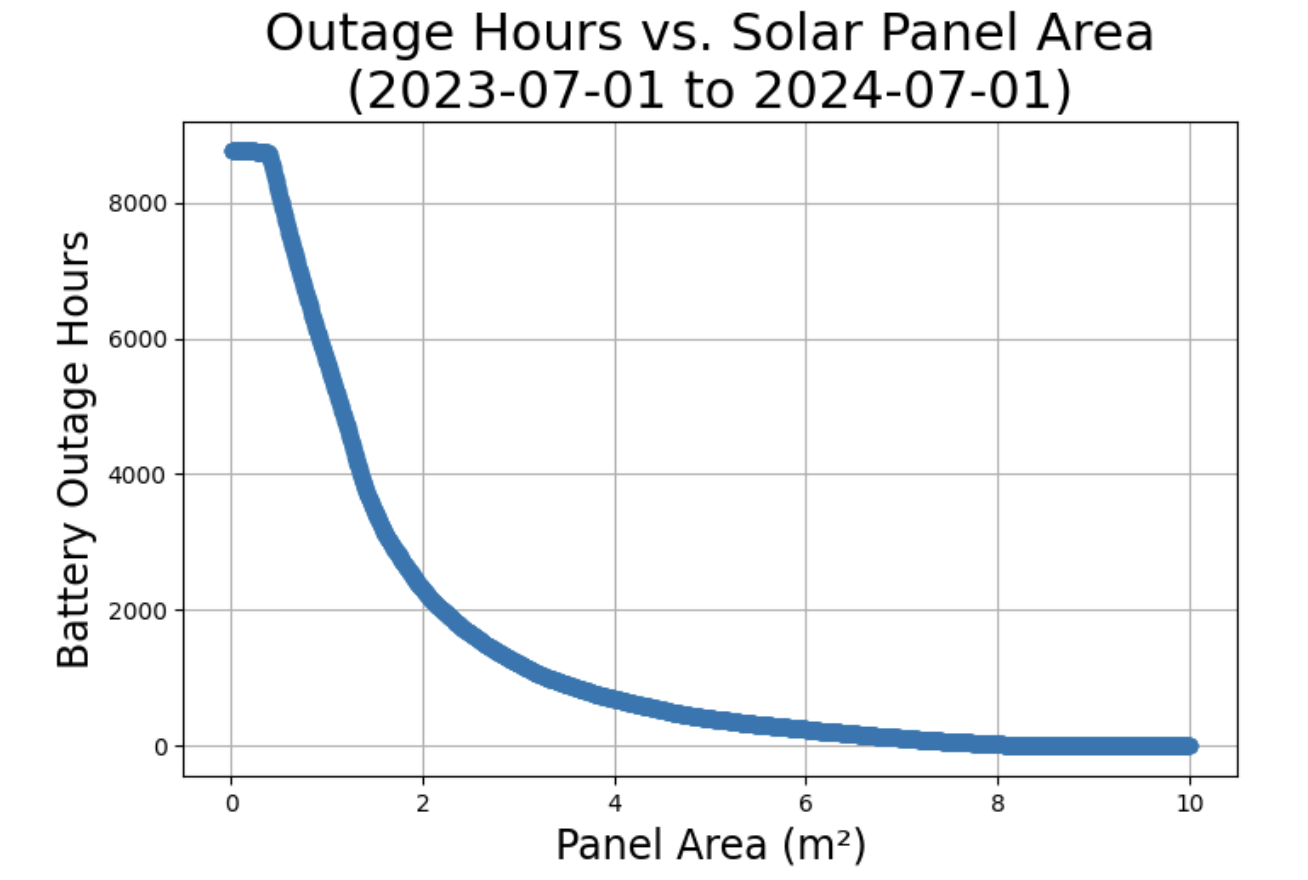
\includegraphics[width=0.95\linewidth]{Model I 3500.png}
\caption{Estimated outage versus solar panel area for a high-capacity battery case from historical irradiance data.}
\label{fig:solar_model}
\end{figure}

The operational implication is straightforward: full winter uptime often requires substantial panel oversizing, so deployments must balance target availability, enclosure footprint, and lifecycle cost.
\subsection{Current limitations and next measurements}
Current results are pilot-scale and cover limited seasonal variability. The next measurement campaign expands to longer windows, richer failure taxonomies, and targeted ablations, including lane polygons with/without wheel refinement and triggered vs non-triggered export latency. As additional annotated windows become available, the same deployment logs can support deeper quantitative analyses without changing the deployed architecture.

Power autonomy remains another practical constraint for distributed deployments \cite{chamola}. We continue to use hourly solar-resource modeling \cite{KHATIB20122864, nasapowerpaper, nasaAPI} to size panel and battery combinations against expected edge load and target uptime.

\section{Conclusion}
AvenaRS provides a deployed, edge-native camera and sensor architecture for lane-level pavement monitoring. The system unifies high-rate acquisition, camera event extraction, semantic message transport, calibration-aware storage, and operator-facing control. Deployment evidence from I-65 and APT indicates that the platform can sustain field workflows for continuity, recovery, and user-directed data access while preserving a clear path to future quantitative expansion.

\balance
\section*{Acknowledgment}
This study is supported by the Joint Transportation Research Program between the Indiana Department of Transportation and Purdue University under SPR-4918.

\bibliographystyle{IEEEtran}
\bibliography{avena_refs}

\end{document}
